%%%%%%%%%%%%%%%%%%%%%%% file template.tex %%%%%%%%%%%%%%%%%%%%%%%%%
%
% This is a general template file for the LaTeX package SVJour3
% for Springer journals.          Springer Heidelberg 2010/09/16
%
% Copy it to a new file with a new name and use it as the basis
% for your article. Delete % signs as needed.
%
% This template includes a few options for different layouts and
% content for various journals. Please consult a previous issue of
% your journal as needed.
%
%%%%%%%%%%%%%%%%%%%%%%%%%%%%%%%%%%%%%%%%%%%%%%%%%%%%%%%%%%%%%%%%%%%
%
% First comes an example EPS file -- just ignore it and
% proceed on the \documentclass line
% your LaTeX will extract the file if required
\begin{filecontents*}{example.eps}
%!PS-Adobe-3.0 EPSF-3.0
%%BoundingBox: 19 19 221 221
%%CreationDate: Mon Sep 29 1997
%%Creator: programmed by hand (JK)
%%EndComments
gsave
newpath
  20 20 moveto
  20 220 lineto
  220 220 lineto
  220 20 lineto
closepath
2 setlinewidth
gsave
  .4 setgray fill
grestore
stroke
grestore
\end{filecontents*}
%
\RequirePackage{fix-cm}
%
%\documentclass{svjour3}                     % onecolumn (standard format)
%\documentclass[smallcondensed]{svjour3}     % onecolumn (ditto)
\documentclass[smallextended]{svjour3}       % onecolumn (second format)
%\documentclass[twocolumn]{svjour3}          % twocolumn
%
\smartqed  % flush right qed marks, e.g. at end of proof
%
\usepackage{graphicx}
%
% \usepackage{mathptmx}      % use Times fonts if available on your TeX system
%
% insert here the call for the packages your document requires
%\usepackage{latexsym}
% etc.
%
% please place your own definitions here and don't use \def but
% \newcommand{}{}
%
% Insert the name of "your journal" with
% \journalname{myjournal}
%

%%%%%%%%%%%%self-define%%%%%%%%%%%%%%%%%%
\usepackage[tight,footnotesize]{subfigure}
\begin{document}

\title{Revolution or Regression?%\thanks{Grants or other notes
%about the article that should go on the front page should be
%placed here. General acknowledgments should be placed at the end of the article.}
}
\subtitle{-A Comparatively Empirical Study of Two Agile Development Processes?\\ If so, write it here}

%\titlerunning{Short form of title}        % if too long for running head

\author{Yujuan Jinag         \and
         Josh Chiang \and
	Roy Budhai \and
	Bram Adams %etc.
}

%\authorrunning{Short form of author list} % if too long for running head

\institute{F. Author \at
              first address \\
              Tel.: +123-45-678910\\
              Fax: +123-45-678910\\
              \email{fauthor@example.com}           %  \\
%             \emph{Present address:} of F. Author  %  if needed
           \and
           S. Author \at
              second address
}

\date{Received: date / Accepted: date}
% The correct dates will be entered by the editor


\maketitle

\begin{abstract}
Insert your abstract here. Include keywords, PACS and mathematical
subject classification numbers as needed.
\keywords{First keyword \and Second keyword \and More}
% \PACS{PACS code1 \and PACS code2 \and more}
% \subclass{MSC code1 \and MSC code2 \and more}
\end{abstract}

%\section{Introduction}
%\label{intro}
%Your text comes here. Separate text sections with
%\section{Section title}
%\label{sec:1}
%Text with citations \cite{RefB} and \cite{RefJ}.
%\subsection{Subsection title}
%\label{sec:2}
%as required. Don't forget to give each section
%and subsection a unique label (see Sect.~\ref{sec:1}).
%\paragraph{Paragraph headings} Use paragraph headings as needed.
%\begin{equation}
%a^2+b^2=c^2
%\end{equation}

% For one-column wide figures use
%\begin{figure}
% Use the relevant command to insert your figure file.
% For example, with the graphicx package use
  %
\includegraphics{example.eps}
% figure caption is below the figure
%\caption{Please write your figure caption here}
%\label{fig:1}       % Give a unique label
%\end{figure}
%
% For two-column wide figures use
%\begin{figure*}
% Use the relevant command to insert your figure file.
% For example, with the graphicx package use
 % 
\includegraphics[width=0.75\textwidth]{example.eps}
% figure caption is below the figure
%\caption{Please write your figure caption here}
%\label{fig:2}       % Give a unique label
%\end{figure*}
%
% For tables use
%\begin{table}
% table caption is above the table
%\caption{Please write your table caption here}
%\label{tab:1}       % Give a unique label
% For LaTeX tables use
%\begin{tabular}{lll}
%\hline\noalign{\smallskip}
%first & second & third  \\
%\noalign{\smallskip}\hline\noalign{\smallskip}
%number & number & number \\
%number & number & number \\
%\noalign{\smallskip}\hline
%\end{tabular}
%\end{table}

\section{Introduction and Motivation}
\label{sec:intro}



\section{Related Work}
\label{sec:relatedWork}



\section{Approach}
\label{sec:appraoch}


\subsection{Select Study Case}
The dominate project P of this company S was launched in 2014 summer. At the beginning, it adopted traditional branch-based integration hierarchy. Since 2015 May, they started adopting a new mechanism-``feature toggling'' in order to improve the integration and testing efficiency. This allows us to compare the two integration approaches in a rather steady context with less independent variables to control. Figure [REF] shows the two different integration approaches in this company.


\subsection{Data Collection}
We collect the data of this project from 2014 May until 2015 September, including the build information from Jenkins, reviewing information from Gerrit and development information from Git. 


\subsection{key Performance Indicators}
We proposed a bunch of KPIs (Key Performance Indicator) to compare the two approaches from different perspectives. After discussing with engineers of this company, we nailed down the four main KPIs covering three dimensions (shown in Table \ref{tab:KPI}). These KPIs are the most important ones from the industry perspective.


\textbf{Integration effort} indicates how difficut to integrate a commit into the main trunk, is measured by the size of merge commits. When a commit is integrated into another branch seamlessly, the size of merge commit will be zero. If a commit causes integration conflicts when being merged into another branch, developer needs to fix the conflicts by modifying integration context. The more code lines are been changed, the larger the merge commit will be. Thus, the size of merge commit can reflect the effort developers spend for integrating a new commit.



\textbf{Productivity} wants to measure if there is difference for development efficiency as well as the amount of developers contributions with \textbf{LOC (Line Of Code)} and \textbf{Success rate}. We sum up LOC of all commits that integrated into main trunk submitted by each developer. Success rate is used to measure how easily a commit get into main trunk. In this project, every code change made by developer needs to be submitted to Gerrit to review. If reviewers think this change needs to be revised, the developer needs to work on it and submitted a new version later. The more versions one commit goes through, the more difficult to accept new code changes. The success rate is defines as the number of commits divided by its corresponding patch revisions. For example, if a code change is accepted the first time it's reviewed, its success rate is 100\%. If a code change is revised once, then its success rate is 50\%.


\textbf{Quality assurance} is measured with the number of bug-fixes per release. In our case study, the branch stable only integrate the bug-fixes commits to stablize the staging release version, so we just need to count the number of commits integrated by stable branch. Note the bug-fixes here are pre-release bug-fixes.



\begin{table}
\caption{The Four most important KPIs.}
\label{tab:KPI}       % Give a unique label
\begin{tabular}{rll}
\hline\noalign{\smallskip}
dimension & KPI   \\
\noalign{\smallskip}\hline\noalign{\smallskip}
Integration Effort & number \\
Productivity & LOC (per developer) \\
 & Success rate \\
Quality Assurance & \# of bugs \\
\noalign{\smallskip}\hline
\end{tabular}
\end{table}


\section{Case Study Result}
\label{sec:result}

\subsection{Integration Effort}

\textbf{Motivation:} 
Which approach makes integration easier?

\textbf{Approach:}
Size of merge commit. Distribution across all merge commits.

\textbf{Findings:} 

\textbf{It is easier to merge branches into main trunk with branch-based approach.} Figure \ref{fig:integrationEffort} is the beanplot of merge commit size distributions for the two period of project for each merge commit. We can see the median value of all merge commits' size is much smaller than that of toggle-based approach. This means it cost less effort to merge sub-branches into main trunk in the branch-based hierarchy. 

\begin{figure*}
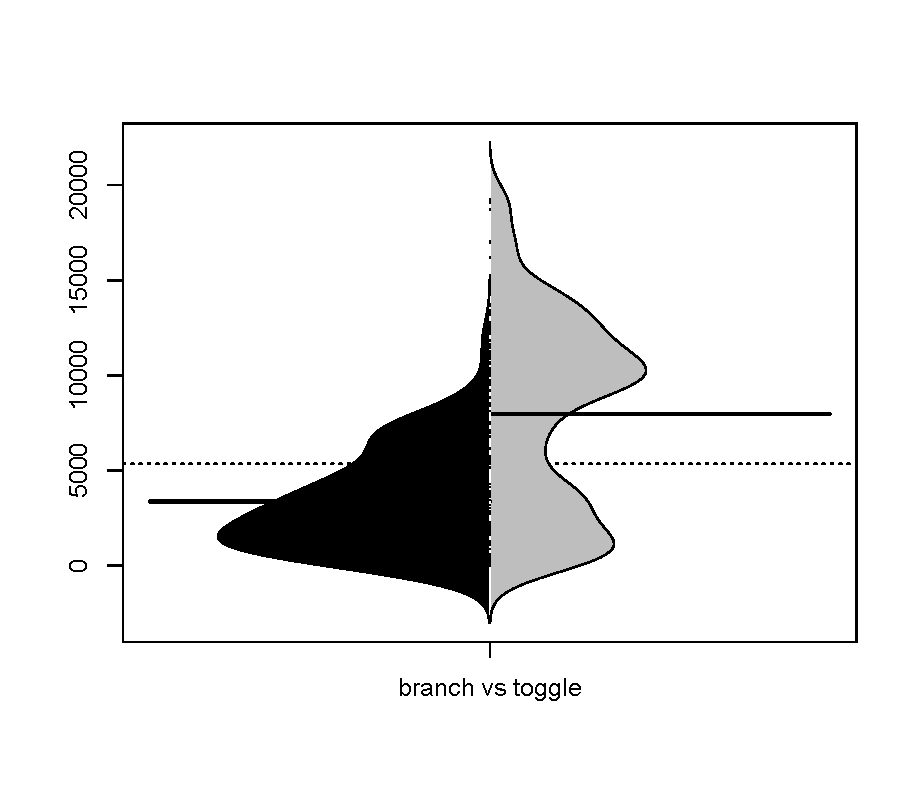
\includegraphics[width=0.95\textwidth]{figure/beforeAfterIE.pdf}
\caption{Beanplot of integration effort.}
\label{fig:integrationEffort}
\end{figure*}


\subsection{Productivity}

\textbf{Motivation:}
Which approach helps developers contribute more code and help code being qualified faster?

\textbf{Approach:}
Sum up LOC for each developer and success rate per commit.

\textbf{Findings:} 

\textbf{There is no difference between two aproaches in terms of developers' contribution.} Figure \ref{fig:LOC} demonstrates the distribution of LOC per developer. We can see the median value of LOC of both approaches do not differ a lot. Toggle-based approach is a bit higher.


\begin{figure*}
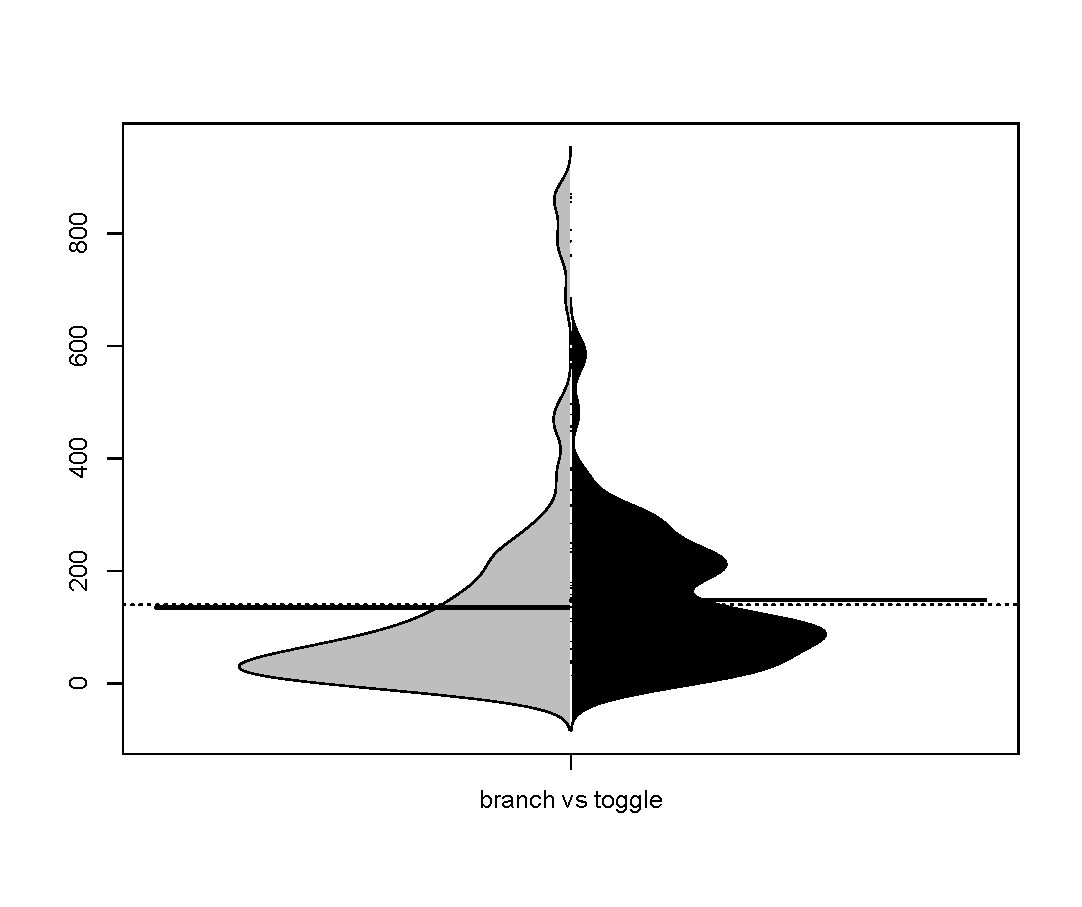
\includegraphics[width=0.95\textwidth]{figure/avgLOC.pdf}
\caption{Beanplot of LOC distribution per developer.}
\label{fig:LOC}
\end{figure*}


\textbf{The number of commits and corresponding patch revisions are increasing while the rate is decreasing.} Figure \ref{subfig:successRateNum} shows the number of integrated commits and its corresponding patch revisions grouped by release. Before 2015-W18 is branch-based approach and after is toggle-based approach. We can see that the number of both increases significantly after adopting toggling mechanism. However, on the other way around the rate decreases. 

\begin{figure*}
    \subfigure[\# of accepted commits and its corresponding patchset revisions]{
	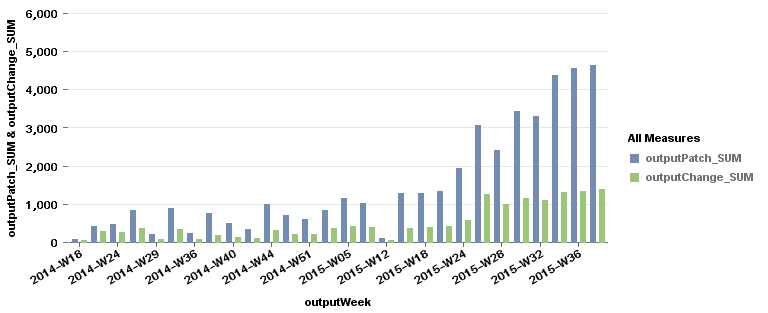
\includegraphics[width=0.95\textwidth]{figure/successRateByRelOrcaNum.png}
	\label{subfig:successRateNum}
    }
    \subfigure[Success rate rate]{
	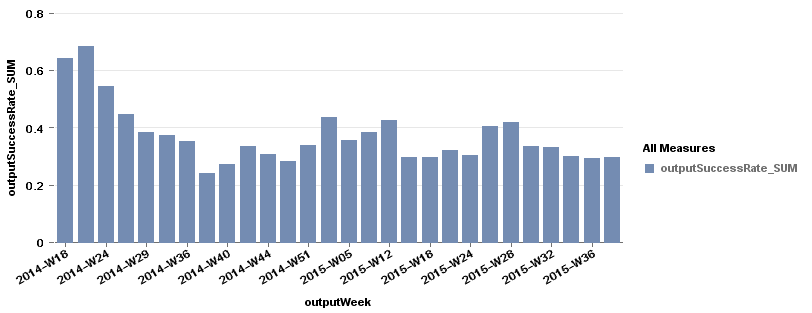
\includegraphics[width=0.95\textwidth]{figure/successRateByRelOrcaRatio.png}
	\label{subfig:successRateRate}
    }
\caption{Success rate and corresponding statistics per release.}
\label{fig:successRate}
\end{figure*}


\subsection{Quality Assurance}

\textbf{Motivation:}
Which approach appeals more pre-release bugs?

\textbf{Approach:}
Count number of bug-fixes per release.

\textbf{Findings:} 

\textbf{Toggle-based approach introduces more bugs.} Figure \ref{fig:bug} shows the distribution of bug-fixes for each approach per day. We found that the median value of distribution of bug-fixes for toggle-based approach is much higher than that of branch-based approach.

\begin{figure*}
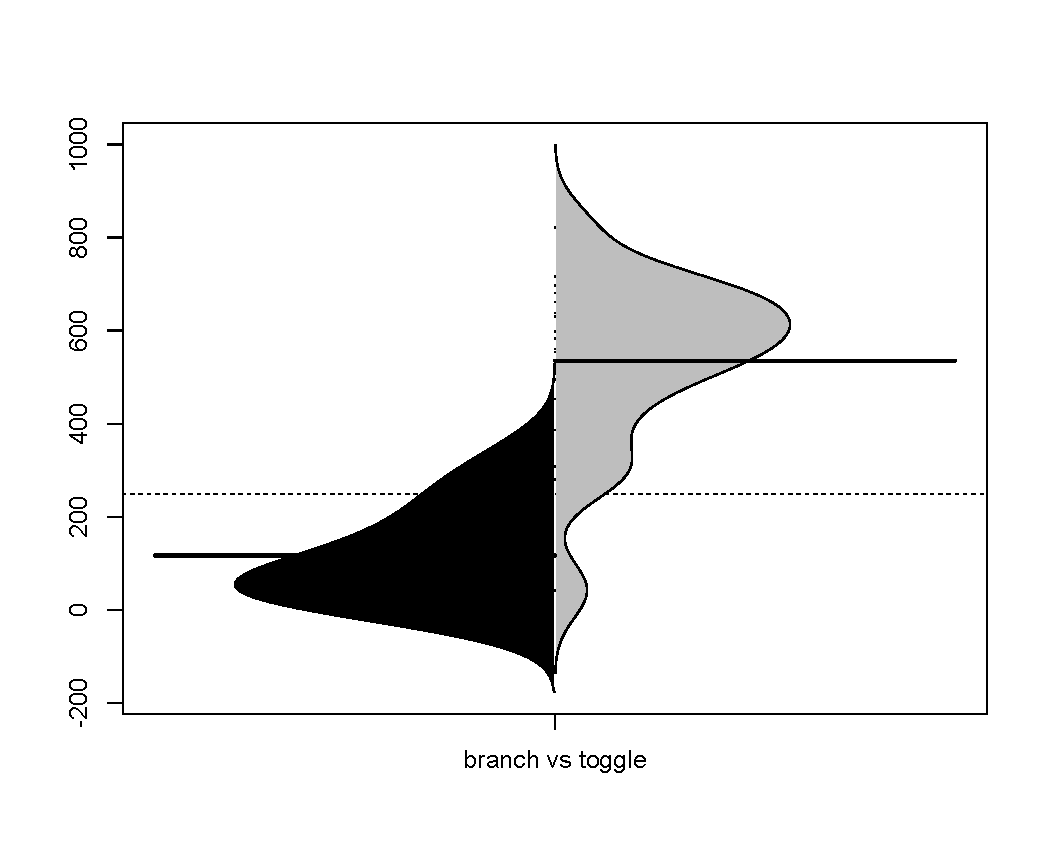
\includegraphics[width=0.95\textwidth]{figure/beforeAfterBug.pdf}
\caption{Beanplot of distributions of bug-fixes.}
\label{fig:bug}
\end{figure*}



\section{Conclusion}

\section{Threats to Validity}

\section{Acknowledgement}





%\begin{acknowledgements}
%If you'd like to thank anyone, place your comments here
%and remove the percent signs.
%\end{acknowledgements}

% BibTeX users please use one of
%\bibliographystyle{spbasic}      % basic style, author-year citations
%\bibliographystyle{spmpsci}      % mathematics and physical sciences
%\bibliographystyle{spphys}       % APS-like style for physics
%\bibliography{}   % name your BibTeX data base

% Non-BibTeX users please use
\begin{thebibliography}{}
%
% and use \bibitem to create references. Consult the Instructions
% for authors for reference list style.
%
\bibitem{RefJ}
% Format for Journal Reference
Author, Article title, Journal, Volume, page numbers (year)
% Format for books
\bibitem{RefB}
Author, Book title, page numbers. Publisher, place (year)
% etc
\end{thebibliography}

\end{document}
% end of file template.tex

